\chapter{Concept for an Exergame for Elderly}


\section{A Video Game Series}
\begin{figure} [ht!]
\centering
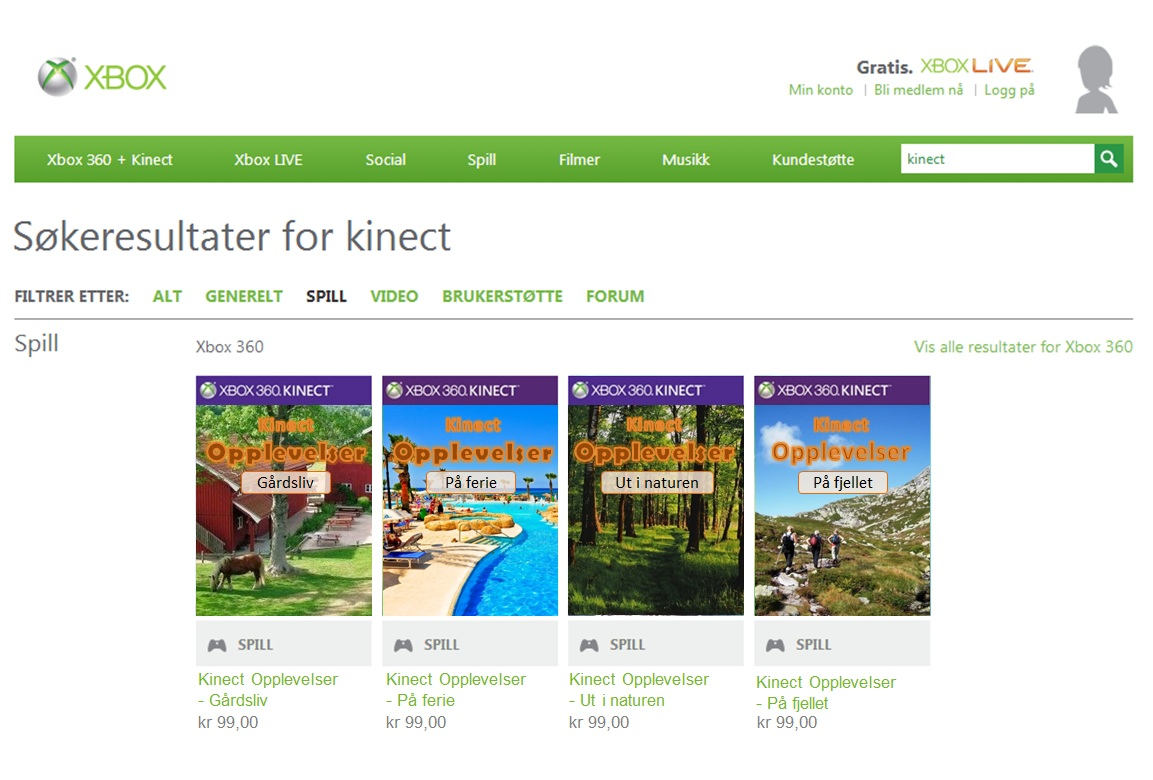
\includegraphics[scale=0.5, angle=90]{SpillXboxNYNY.jpg}
\caption[Presentation of our video game series]{A presentation of how our video game series would look like on Xbox's website [modified from \cite{XboxNettside}].}
\label{fig:videogameseriesHele}
\end{figure}



\section{Out in the Nature}

\begin{figure} [ht!]
\centering
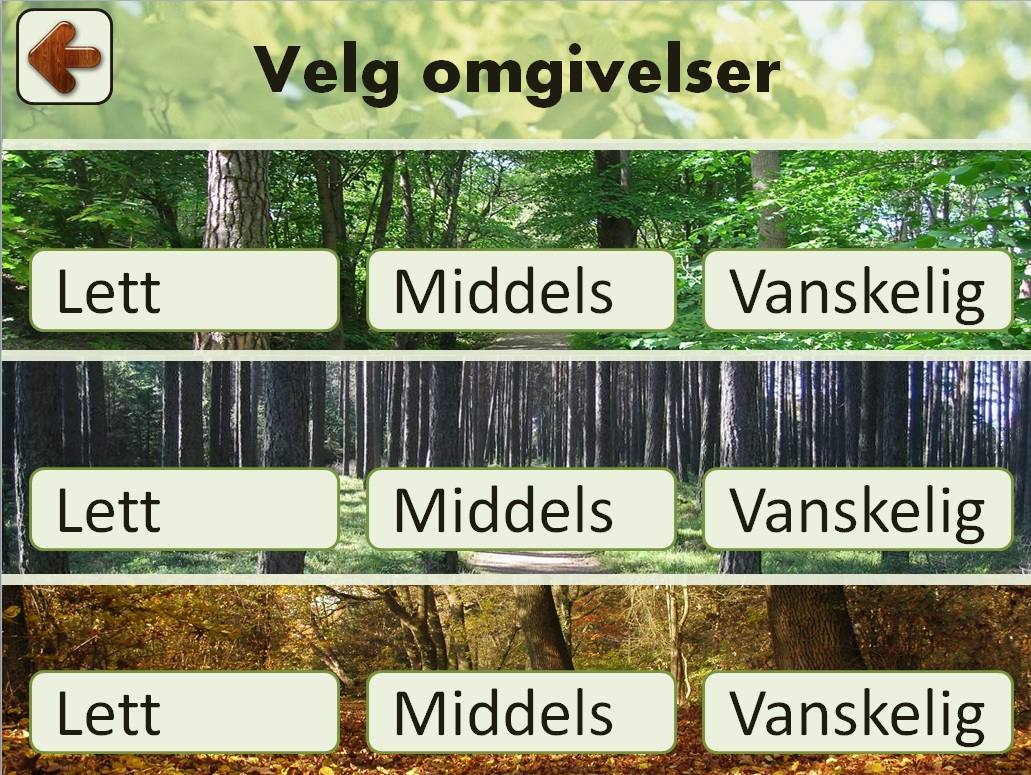
\includegraphics[scale=0.45]{VelgOmgivelser.jpg}
\caption[Choice of surroundings and difficulty]{When "Take a walk in the nature" is chosen, players will get the possibility to choose surroundings and difficulty level.}
\label{fig:omgivelseNivaa}
\end{figure}

\begin{figure} [ht!]
\centering
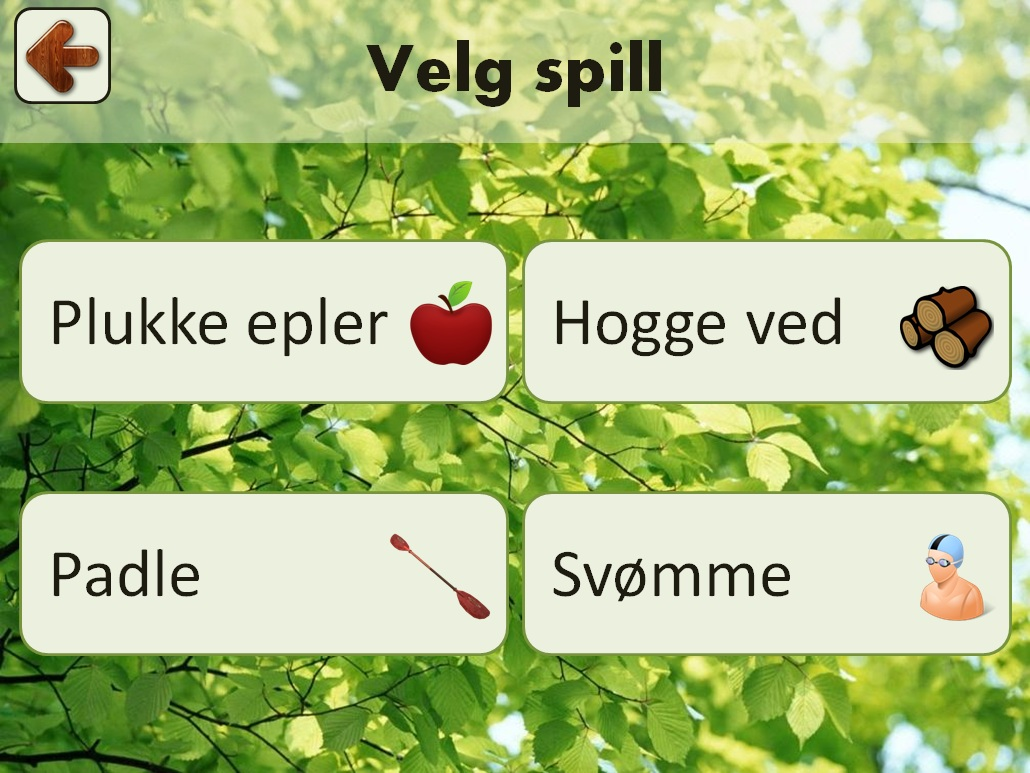
\includegraphics[scale=0.4]{VelgSpill.jpg}
\caption[The four single games]{Besides the walk in the nature the players can choose between four single games, picking apples, chopping wood, paddling, and swimming.}
\label{fig:velgSpill}
\end{figure}


\section{The Menu}

One of the main problems we observed during workshop 1 was related to handling the menus in the different games. The general perception from workshop 1, in addition to our own experience from playing, was that the menus were complex, difficult to follow, demanding to navigate through, and that they were too sensitive. Therefore, we have made a prototype for a menu, which we will present in this section. The menu prototype is developed with Microsoft PowerPoint.

The design of our menu proposal is based upon feedback from workshop 1, and theory about designing interfaces for elderly. Simple design, distinct elements, and easy to read information is emphasised to make it user-friendly for elderly that might suffer from declined vision. It has been a focus not to have too much information in each menu step. We have therefore chosen to make a menu consisting of more steps, rather than filling few menu steps with lots of information and choices.   

Figure \ref{fig:velgSpill} shows one step of the menu and the different menu elements. We have used a range of green colors, and a picture of green leaves as background, to create a theme related to forest and nature. Menu buttons are arranged as list elements or in a square, depending on what is most appropriate. The size of the elements are chosen with usability in mind, there should be room for a proper font size, and it should be easy to push the right button. The buttons have a light green, almost white, background color, with a darker green outline. The text is written in black with an easy-to-read font. The contrast between button background and text color is chosen with respect to design guidelines for elderly, presented in Section \ref{sec:designelderly}. The chosen colors is also based \cite{blindeforbundetTekst}. Taking the element's surroundings into account when choosing colors is important if you will make the element stand out. With e.g. green vegetation as surroundings, white background color and black, dark green, or dark blue text should be chosen to create maximum contrast.   

The title on each step is written in a bold, black, easy to read font, on a semi-transparent light-colored background. The title is stating what choice to be made at the current step. From the Eight Golden Rules presented in Section \ref{sec:designguide} we know that it is important to have an interface with visible information. These rules also says that users always should be given feedback on their actions. In addition to this, from workshop 1 there was a general opinion that the informants wanted to see response on their actions. We have included this in our concept by portraying hand movements with a avatar hand, and by highlighting elements that are "in action", see Figure blabla.   

Up in the left corner there is a back button, which will make it possible for users to always regret their action. The permission to reverse actions is also an important guideline from the Eight Golden Rules. The back button is shaped and colored as the other menu buttons to maintain consistency and intuitiveness. The choice of placement is based on guidelines stating that navigation should be on top, and on the natural way to read and observe information, which is from top to bottom, from left to right [KILDEee]. We avoided placing the back button in the bottom left corner to not mix it with the cancel/pause feature included in the Kinect software (holding your left hand straight 45 degrees from your body). The back button is marked with a wooden arrow, a familiar and intuitive icon related to navigation. The choice of using an wooden arrow is based on its relation to our forest theme. 
       
Farger.
Lys bakgrunn, mørk tekst.
Blad som bakgrunn.
Kontraster i forhold til omgivelsene. 

\begin{figure} [ht!]
\centering
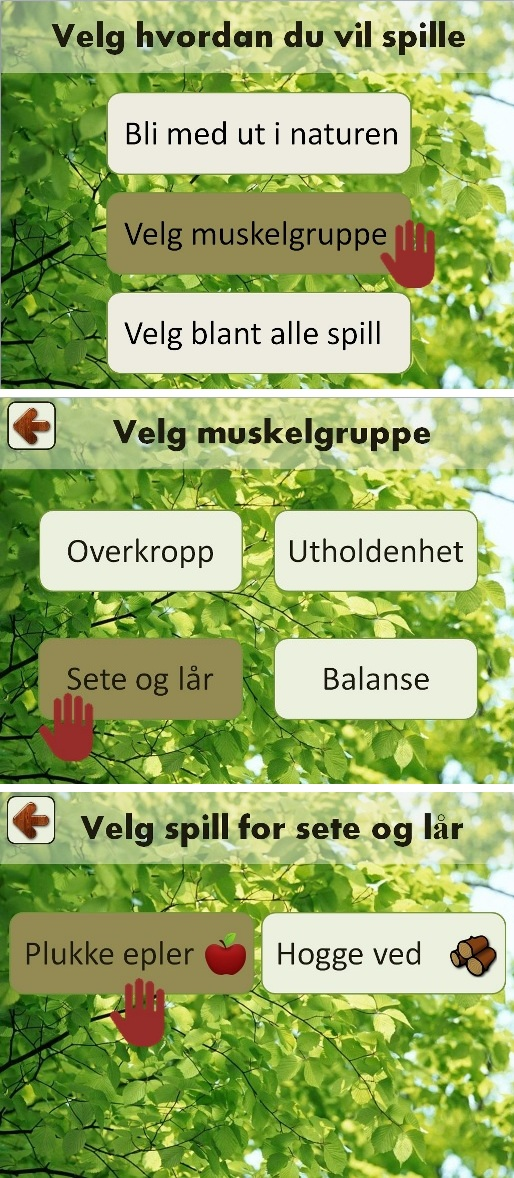
\includegraphics[scale=0.5]{menuStep1.jpg}
\caption[The menu, part one]{This figure shows the menu step by step, from the beginning to playing a single game, here picking apples. The selection of single games is a result of the chosen muscle group.}
\label{menu1}
\end{figure}

\begin{figure} [ht!]
\centering
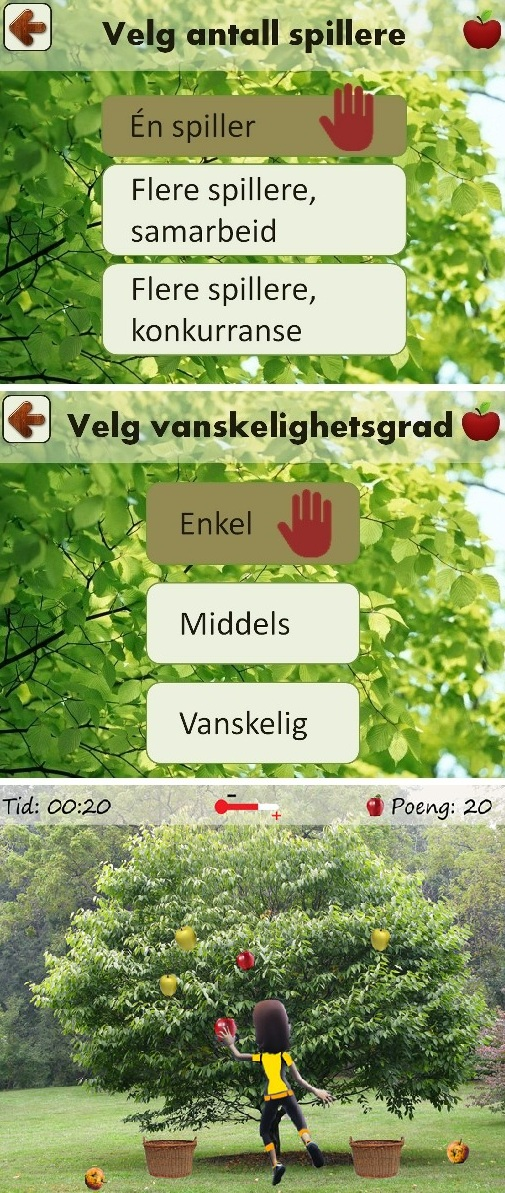
\includegraphics[scale=0.5]{menuStep2.jpg}
\caption[The menu, part two]{This figure shows the menu step by step, from the beginning to playing a single game, here picking apples. Single player game and difficulty level easy are chosen.}
\label{menu2}
\end{figure}

\section{Miscellaneous Aspects to Consider About the Concept}